\subsection{Constructions}\label{sec:naysayer_apps}

In \Cref{sec:merkle_naysayer}, we show a concrete example of the generic naysayer construction from \Cref{thm:naysayer} applied to Merkle trees. We then highlight three naysayer proof constructions which take advantage of repetition in the verification algorithm to achieve better naysayer performance: the FRI polynomial commitment scheme (\Cref{sec:fri_naysayer}) and two post-quantum signature schemes (\Cref{sec:pqsig_naysayer}). 
% In this section, we highlight three naysayer proof constructions which take advantage of such repetition to achieve better performance: the FRI polynomial commitment scheme (\Cref{sec:fri_naysayer}) and two post-quantum signature schemes (\Cref{sec:pqsig_naysayer}). 
Then, in \Cref{sec:vshuffle_naysayer}, we give an example of a non-public naysayer proof which uses a trapdoor to reduce the size and verification complexity of the naysayer proof. %\todo{as well as its computation complexity?}.
Finally, in \Cref{sec:eval} we
% summarize the succinctness of each naysayer proof compared to that of the original proof system.
estimate the performance of each naysayer proof system compared to that of the original proof system.

\subsubsection{Merkle Commitments}\label{sec:merkle_naysayer}
\begin{figure*}[tb]
    \centering
    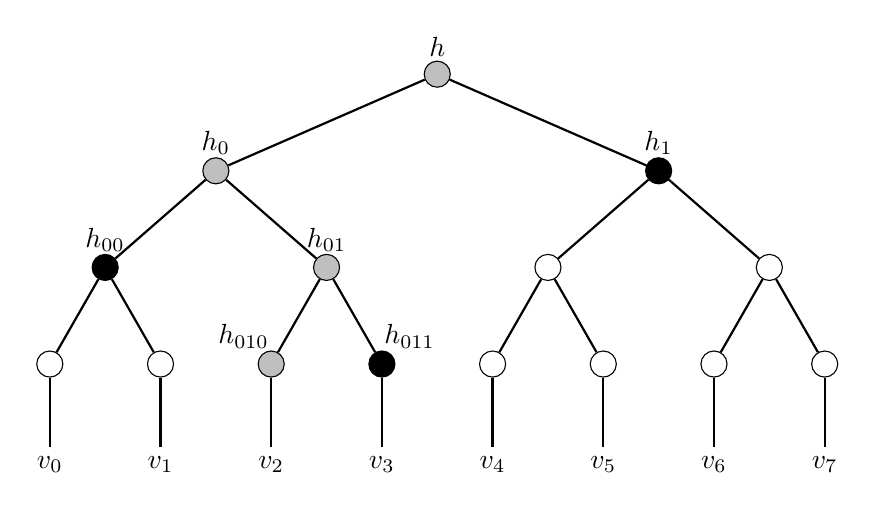
\begin{tikzpicture}[par/.style={sloped,fill=white,inner sep=-.4ex}]
    \tikzstyle{circ} = [circle, draw]
    \tikzstyle{path} = [circle, draw, fill=lightgray]
    \tikzstyle{copath} = [circle, draw, fill=black]
        \node[path] (root) {};
        % level 1
        \node[path,below=3em,xshift=-8em] (l) at (root) {};
        \node[copath,below=3em,xshift=8em] (r) at (root) {};
        \draw[-,thick] (l) -- (root);
        \draw[-,thick] (r) -- (root);
        % level 2
        \node[copath,below=3em,xshift=-4em] (ll) at (l) {};
        \node[path,below=3em,xshift=4em] (lr) at (l) {};
        \draw[-,thick] (ll) -- (l);
        \draw[-,thick] (lr) -- (l);
        \node[circ,below=3em,xshift=-4em] (rl) at (r) {};
        \node[circ,below=3em,xshift=4em] (rr) at (r) {};
        \draw[-,thick] (rl) -- (r);
        \draw[-,thick] (rr) -- (r);
        % level 3
        \node[circ,below=3em,xshift=-2em] (lll) at (ll) {};
        \node[circ,below=3em,xshift=2em] (llr) at (ll) {};
        \draw[-,thick] (lll) -- (ll);
        \draw[-,thick] (llr) -- (ll);
        \node[path,below=3em,xshift=-2em] (lrl) at (lr) {};
        \node[copath,below=3em,xshift=2em] (lrr) at (lr) {};
        \draw[-,thick] (lrl) -- (lr);
        \draw[-,thick] (lrr) -- (lr);
        \node[circ,below=3em,xshift=-2em] (rll) at (rl) {};
        \node[circ,below=3em,xshift=2em] (rlr) at (rl) {};
        \draw[-,thick] (rll) -- (rl);
        \draw[-,thick] (rlr) -- (rl);
        \node[circ,below=3em,xshift=-2em] (rrl) at (rr) {};
        \node[circ,below=3em,xshift=2em] (rrr) at (rr) {};
        \draw[-,thick] (rrl) -- (rr);
        \draw[-,thick] (rrr) -- (rr);
        % leaves
        \node[below=3em] (0) at (lll) {$v_0$};
        \draw[-,thick] (0) -- (lll);
        \node[below=3em] (1) at (llr) {$v_1$};
        \draw[-,thick] (1) -- (llr);
        \node[below=3em] (2) at (lrl) {$v_2$};
        \draw[-,thick] (2) -- (lrl);
        \node[below=3em] (3) at (lrr) {$v_3$};
        \draw[-,thick] (3) -- (lrr);
        \node[below=3em] (4) at (rll) {$v_4$};
        \draw[-,thick] (4) -- (rll);
        \node[below=3em] (5) at (rlr) {$v_5$};
        \draw[-,thick] (5) -- (rlr);
        \node[below=3em] (6) at (rrl) {$v_6$};
        \draw[-,thick] (6) -- (rrl);
        \node[below=3em] (7) at (rrr) {$v_7$};
        \draw[-,thick] (7) -- (rrr);
        %%% labels
        % path
        \node[yshift=1em] at (root) {$h$};
        \node[yshift=1em] at (l) {$h_0$};
        \node[yshift=1em] at (lr) {$h_{01}$};
        \node[yshift=1em,xshift=-1em] at (lrl) {$h_{010}$};
        % copath
        \node[yshift=1em] at (r) {$h_1$};
        \node[yshift=1em] at (ll) {$h_{00}$};
        \node[yshift=1em,xshift=1em] at (lrr) {$h_{011}$};
    \end{tikzpicture}
    \caption{Each node in a Merkle tree consists of a hash of its children. The root $h$ is a commitment to the vector of leaves $(v_0, v_1, \dots, v_7)$. An opening proof for the element $v_2$ is its copath (black nodes); the ``verification trace'' for the proof is the path (gray nodes).}
    \label{fig:merkle-diagram}
\end{figure*}

Merkle trees~\cite{C:Merkle87} and their variants are ubiquitous in modern systems, including Ethereum's state storage~\cite{ethereum_trie}. A Merkle tree can be used to commit to a vector $\vec{v}$ of elements as shown in \Cref{fig:merkle-diagram}, with the root $h$ acting as a commitment to $\vec{v}$. The party who created the tree can prove the inclusion of some element $v_i$ at position $i$ in the tree by providing the corresponding copath. 

For example, to open the leaf at position 2, a prover provides its value $v_2$ and an opening proof $\pi = (h_{011}, h_{00}, h_{1})$ consisting of the copath from the leaf $v_2$ to the root $h$. The proof $\pi$ is checked by using its contents to recompute the root $h'$ starting with $v_2$, then checking that $h = h'$. This involves recomputing the nodes along the path from the leaf to the root (the blue nodes in the figure). These nodes can be seen as a ``verification trace'' for the proof $\pi$.
    
In the context of a naysayer proof system, the prover provides $\pi$ along with the verfication trace $\aux = (h_{010}, h_{01}, h_{0})$. A naysayer can point out an error at a particular point of the trace by submitting the incorrect index of $\aux$ (e.g., $\pi_\nay = 1$ to indicate $h_{01}$). The naysayer verifier checks $\pi_\nay$ by computing a single hash using $\pi$ and oracle access to $\aux$, e.g., checking $H(h_{010}, h_{011}) \stackrel{?}{=} h_{01}$, where $h_{010}, h_{01} \in \aux$ and $h_{011} \in \pi$. This is the generic construction from \Cref{thm:naysayer}.

\subsubsection{FRI}\label{sec:fri_naysayer}

The Fast Reed-Solomon IOP of proximity (FRI)~\cite{ICALP:BBHR18} is used as a building block in many non-interactive proof systems, including the STARK IOP~\cite{EPRINT:BBHR18}.
Below, we describe only the parts of FRI as applied in STARK. We refer the reader to the cited works for details.

The FRI commitment to a polynomial $p(X)\in\FF[X]^{\leq d}$ is the root of a Merkle tree with $\rho^{-1}d$ leaves. 
Each leaf is an evaluation of $p(X)$ on the set $L_0 \subset \FF$, where $\rho^{-1}d=\sizeof{L_0} \ll \sizeof{\FF}$ for a constant $0<\rho<1$ (the Reed-Solomon rate parameter). We focus on the verifier's cost in the proof of proximity. Let $\delta$ be a parameter of the scheme such that $\delta\in(0,1-\sqrt{\rho})$. The prover sends $\log{d}+1$ values (roots of successive ``foldings'' of the original Merkle tree, plus the value of the constant polynomial encoded by the final tree). The verifier makes $q=\secpar/\log(1/(1-\delta))$ queries to ensure $2^{-\secpar}$ soundness error; the prover responds to each query with $2\log{d}$ Merkle opening proofs (2 for each folded root). For each query, the verifier must check each Merkle authentication path, amounting to $\bigO{\log{\rho^{-1}d}}$ hashes per query. Furthermore, it must perform $\log{d}$ arithmetic checks (roughly 3 additions, 2 divisions, and 2 multiplications in $\FF$) per query to ensure the consistency of the folded evaluations. Therefore, the overall FRI verification consists of $\bigO{\secpar\log{d}}$ hashes and field operations.

A FRI proof is invalid if any of the above checks fails. Therefore a straightforward naysayer proof $\pi^{\mathsf{FRI}}_{\nay}=(i,j,k)$ need only point out a single Merkle proof (the $j$th proof for the $i$th query, $i\in[q], j \in [2\log{d}]$) or a single arithmetic check $k \in [q\log{d}]$ which fails. The naysayer verifier only needs to recompute that particular check: $\bigO{\log{\rho^{-1}d}}$ hashes in the former case\footnote{One could use a Merkle naysayer proof (\Cref{sec:merkle_naysayer}) to further reduce the naysayer verification from checking a full Merkle path to a single hash evaluation.} or a few arithmetic operations over $\FF$ in the latter.

\subsubsection{Post-quantum Signature Schemes}\label{sec:pqsig_naysayer}

With the advent of account abstraction~\cite{accountabstraction}, Ethereum users can define their own preferred digital signature schemes, including post-quantum signatures as recently standardized by NIST~\cite{CCS:BHKNRS19,TCHES:DKLLS18,NISTPQC:FALCON22}.
Compared to their classical counterparts, post-quantum signatures generally have either substantially larger signature sizes or substantially larger public key sizes.\footnote{Considering the NIST-standardized post-quantum signature schemes, Dilithium has 1.3KB public keys and 2.4KB signatures for the lowest provided security level (NIST level 2)~\cite{dilithium-spec}; the ``small'' variant of SPHINCS+ for NIST level 1 has 32B public keys but 7.8KB signatures~\cite{sphincsplus-spec}; and FALCON at level 1 has 897B public keys and 666B signatures~\cite{falcon-spec}. By comparison, 2048-bit RSA requires 256B both for public keys and signatures and offers comparable security~\cite{keylength} (only against classical adversaries, of course).}
Since this makes post-quantum signatures expensive to verify on-chain, these schemes are prime candidates for the naysayer proof paradigm.

\paragraph{CRYSTALS-Dilithium~\cite{TCHES:DKLLS18}.} We give a simplified version of signature verification in lattice-based signatures like CRYSTALS-Dilithium. In these schemes, the verifier checks that the following holds for a signature $\sigma=(\vec{z}_1,\vec{z}_2,c)$, public key $\pk=(\vec{A},\vec{t})$, and message $M$:
\begin{equation}\label{eq:crystals_verifier_check}
    \norm{\vec{z}_1}_\infty < \beta \land
    \norm{\vec{z}_2}_\infty < \beta \land 
    c=H(M, \vec{w}, \pk).
\end{equation}
Here $\beta$ is a constant, $\vec{A}\in R_q^{k\times \ell}$, $\vec{z}_1 \in R_q^\ell$, $\vec{z}_2,\vec{t}\in R_q^k$ for the polynomial ring $R_q:=\ZZ_q[X]/(X^d+1)$, and $\vec{w} = \vec{A}\vec{z}_1+\vec{z}_2-c\vec{t} \mod{q}$. (Dilithium uses $d=256$.) We will write elements of $R_q$ as polynomials $p(X) = \sum_{j\in[d]} \alpha_j X^j$ with coefficients $\alpha_j \in \ZZ_q$.
Since \Cref{eq:crystals_verifier_check} is a conjunction, the naysayer prover must show that
\begin{equation}\label{eq:crystals_naysayer_prover}
    \left( \exists z_i \in \vec{z}_1,\vec{z}_2: \norm{z_i}_\infty > \beta \right) \lor 
    c\neq H(M, \vec{w}, \pk).
\end{equation}
If the first check of \Cref{eq:crystals_verifier_check} fails, the naysayer gives an index $i$ for which the infinity norm of one of the polynomials in $\vec{z}_1$ or $\vec{z}_2$ is large. (In particular, it can give a tuple $(b,i,j)$ such that $\alpha_j > \beta$ for $z_i = \dots + \alpha_j X^j + \dots \in \vec{z}_b$.)\footnote{The same idea can be applied to constructions bounding the $\ell_2$ norm, but with lower efficiency gains for the naysayer verifier, who must recompute the full $\ell_2$ norm of either $\vec{z}_1,\vec{z}_2$.}

If the second check fails, the naysayer indicates that clause to the naysayer verifier, who must recompute $\vec{w}$ and perform a single hash evaluation which is compared to $c$.

Overall, $\pi_\nay$ is a tuple $(a, b, i, j)$ indicating (respectively) a clause $a \in [2]$ of \Cref{eq:crystals_naysayer_prover}, the vector $\vec{z}_b$ with $b \in [2]$, an entry $i \in [\max{k,\ell}]$ in that vector, and the index $j \in [d]$ of the coefficient of the ring element at that entry. Since $k \geq \ell$, overall $\sizeof{\pi_\nay} = (2+\log{k}+\log{d})$ bits. The verifier is very efficient when naysaying the first clause, and only slightly faster than the original verifier for the second clause.

\paragraph{SPHINCS+~\cite{CCS:BHKNRS19}.} \todo{proof this paragraph} The signature verifier in SPHINCS+ checks several Merkle authentication proofs, requiring hundreds of hash evaluations. An efficient naysayer proof can be easily devised akin to the naysayer proof described in~\Cref{sec:fri_naysayer}. The naysayer prover simply points to the hash evaluation in one of the Merkle-trees where the signature verification fails. 

\subsubsection{Verifiable Shuffles}\label{sec:vshuffle_naysayer}
Verifiable shuffles are applied in many (blockchain) applications such as single secret leader election algorithms~\cite{AFT:Boneh20}, mix-nets~\cite{CACM:Chaum81}, cryptocurrency mixers~\cite{EPRINT:SNBB19}, and e-voting~\cite{USENIX:Adida08}. The state-of-the-art proof system for proving the correctness of a shuffle is due to Bayer and Groth~\cite{EC:BayGro12}. Their proof system is computationally heavy to verify on-chain as the proof size is $\mathcal{O}(\sqrt{n})$ and verification time is $\mathcal{O}(n)$, where $n$ is the number of shuffled elements. 

Most shuffling protocols (of public keys, re-randomizable commitments, or ElGamal ciphertexts) admit a particularly efficient naysayer proof if the naysayer knows at least one of the shuffled elements. Let us consider the simple case of shuffling public keys. The shuffler wishes to prove membership in the following  NP language:
\begin{align*}%\label{eq:permlanguage}
    \Lang_{perm}:= \{ ((\pk_i,\pk_i')_{i=1}^n,R) : \exists r,\witness_1,\dots,\witness_n \in \FF_p, \sigma \in\mathsf{Perm}(n) \\
    \suchthat \forall i\in[n], \pk_i = g^{\witness_i} \land \pk_i' = g^{r \cdot \witness_{\sigma(i)}} \land R = g^r
    \}.
\end{align*}
Here $\mathsf{Perm}(n)$ is the set of all permutations $f:[n]\rightarrow[n]$.

Suppose a party knows that for some $j\in[n]$, the prover did not correctly include $\pk_j' = g^{r\cdot \witness_j}$ in the shuffle. The party can naysay by showing that 
\[
    (g,\pk_j,R,\pk_j')\in\Lang_{DH}\land \pk_j' \notin (\pk_i,\cdot)_{i=1}^n
\]
where $\Lang_{DH}$ is the language of Diffie-Hellman tuples\footnote{Membership in $\Lang_{DH}$ can be shown via a proof of knowledge of discrete logarithm equality~\cite{C:ChaPed92}.}. To produce such a proof, however, the naysayer must know the discrete logarithm $\witness_j$. Unlike our previous examples, which were public naysayer proofs, this is an example of a private $\naysay$ algorithm using $\td_\nay := \witness_j$. The naysayer proof is $\pi_\nay := (j, \pk_j', \pi_{DH})$. The Diffie-Hellman proof can be checked in constant time and, with the right data structure for the permuted list (e.g., a hash table), so can the list non-membership. This, $\pi_\nay$ is a $\bigO{\log{n}}$-sized naysayer proof with $\bigO{1}$-verification, yielding in exponential savings compared to verifying the original Bayer-Groth shuffle proof.

\subsubsection{Evaluation}
\todo{pick up from here}
We evaluate the asymptotic cost savings for the verifiers in the four examples discussed in \Cref{sec:fri_naysayer,sec:pqsig_naysayer,sec:vshuffle_naysayer}. Note that naysayer proofs allow an exponential speedup for the verifier for verifiable shuffles and a logarithmic speedup for the FRI polynomial commitment opening proof verifier, see~\Cref{tab:apps_table}. For CRYSTALS-Dilithium, we can only claim weakly efficient naysayer proofs, as there is no asymptotic gap in the complexity in certain branches of the signature verification circuit and the naysayer prover algorithm, cf.~\Cref{eq:crystals_verifier_check,eq:crystals_naysayer_prover}.

%------------------BEGIN Naysayer cost savings TABLE--------------
%-----------------------------------------
\begin{table}[tbh!]
   \centering
   \makebox[\linewidth]{
    \setlength{\belowbottomsep}{6pt}
    \begin{tabular}{l c c c c} 
    \toprule
     & \textbf{FRI Opening} & \textbf{CRYSTALS-D.} & \textbf{SPHINCS+}& \textbf{Shuffle proof} \\ [0.5ex] 
     \midrule
     $\pi$ storage & $\mathcal{O}(\secpar\log^2(d))\mathbb{H}$\ & $\mathcal{O}(\secpar)\FF$\  & $\mathcal{O}(\secpar)\FF$\  & $\mathcal{O}(\sqrt{n})\GG$\  \\ 
     $\vrfy(\pi)$ compute & $\mathcal{O}(\secpar\log^2(d))\mathbb{H}$\ & $\mathcal{O}(\secpar)\FF+1\mathbb{H}$\  & $\mathcal{O}(\secpar)\mathbb{H}$\  & $\mathcal{O}(n)\GG$\  \\\midrule
     $\pi_{nay}$ storage & $1\FF$\ & $1\FF\lor1\FF\lor1\FF$\  & $1\FF$\  & $2\GG+1\FF$\  \\
     ${\sf N}\vrfy(\pi_{nay})$ compute & $1\mathbb{H}$\ & $\mathcal{O}(\secpar)\FF\lor\mathcal{O}(\secpar)\FF\lor1\mathbb{H}$\  & $1\mathbb{H}$\  & $4\GG$\  \\
    \bottomrule
    \end{tabular}
    }
    \caption{Cost savings of the naysayer paradigm for the example applications in~\Cref{sec:naysayer_apps}. In FRI, let $deg(p(x))=d$. For the Bayer-Groth shuffle argument~\cite{EC:BayGro12}, we consider $n$ shuffled public keys (or ciphertexts). $\FF,\GG$ denotes field/group elements or field/group operations, respectively. $\mathbb{H}$ denotes hashing operations. \todo{Can I get some estimated numbers here by looking at the implementations/papers of the underlying schemes, and then just the field/group element sizes in the relevant curves for the naysayer?}}
    \label{tab:apps_table}
   \end{table}
   %--------------------END Naysayer cost savings TABLE--------------
   %-------------------------------------------------
   

\noemi{Notice that the naysayer proof consists of an \emph{integer} index (which may only require a few bits to represent). So, even though it is asymptotically logarithmic, in fact it may actually be smaller than many ``regular'' proofs which consist of some group elements (which are normally at least $\secpar$ bits long). -- Need to check this with some common circuit sizes (e.g., the STARK verification circuit) and group element sizes (e.g., BN254 curve G1 element or other).}